\section{Motivation and Approach}
\label{sec:setup}

\begin{figure}
  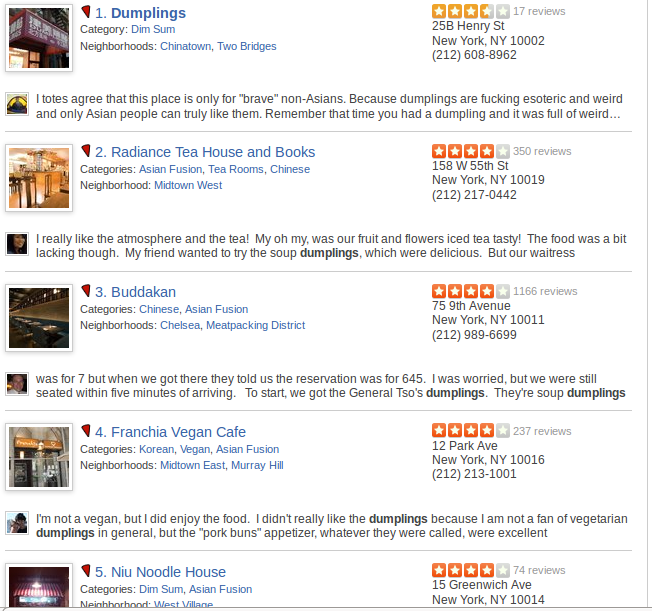
\includegraphics[width=0.5\textwidth]{fig/yelp.png}
  \caption{Yelp search results for "dumplings".
  Most of the top results have 4 stars, forcing users to read lengthy
  review text in order to gain better insight into quality.}
  \label{fig:yelp}
\end{figure}

Given a repository of social media data on a set of physical establishments,
the problem we address in this paper is how to best order establishments in 
a \emph{comparable category}.
Comparable categories are defined by a price point, type of restaurant, and coarse location.
For example, the Doughnut Plant in the Lower East Side would be categorized as <\$, donut\_shop, NYC>.
Per Se in Columbus Circle would be categorized as <\$\$\$\$, french\_restaurant, NYC>.
The type and price annotations are taken directly from Google Maps.

We cast our problem as a machine learning problem.
Social media attributes (e.g. review counts, ratings, check-in counts) are encoded as
features for each particular establishment.
A classifier or regressor model can then be trained to output quality scores for any
establishment. 
The model would output a discrete numerical value, which can be used to later
order places in a comparable category.
However the question remains, how should a training set be labeled
and what should be used as the absolute truth in quality judgement?

One approach is to directly use the average rating from all reviews of a place.
At first glance, using average review score may seem like an attractive
metric to directly use for ranking restaurants.
It is computationally inexpensive, easy to implement, compatible with
most search architectures, and provides significant information gain.
However, it comes with unacceptable long-term consequences:
\squishlist
\item {\bf Reinforcement of popular places} \\
Existing popular places are reinforced at the top of search results \cite{cho2004,cho2005}.
While this has been effectively used to improve Web search results \cite{xue2004},
its use in location-based search may make new high-quality places hard to discover.
This property leads to a substantial bias towards places that were first to become popular,
leading to sparse reviews for other places.
\item {\bf Low resolution of rating} \\
Rating systems tend to be very low resolution (i.e. a single rating from 0-5).
Websites struggle over the tradeoff between keeping the process simple and easy-to-use,
and gaining higher resolution into the different aspects of quality, such as food, service, and decor.
For this reason, a small Chinese dumpling shop in Chinatown has more reviews and the same number
of stars as one of the most critically-acclaimed restaurants in New York City.
It becomes unclear what does 4.5/5.0 stars mean.
A restaurant may have very high food quality, but offer a poorly decorated space.
A salon may offer fantastic service, but at an unreasonably high price.
\item {\bf Noisy data} \\
Users are notoriously inconsistent with their ratings \cite{chevalier2003effect}.
A single bad experience may lead a user to give an establishment 1 star, even when
the restaurant is on average reasonably good.
Additionally, each user has different personal interpretations of the meaning of each rated star,
leading to substantial noise in the final rating.
\squishend

Editorial rating services such as Zagat and Michelin address these limitations in a number of ways.
First, the decision to review a place is not directed by which places they have previously reviewed,
leading to a more even distribution of reviews among establishments.
Second, many provide greater insight into the components of quality with great resolution.
For example, Zagat produces an individual score from 0 to 30 separately for food, service, and decor.
Third, reviews are determined through a very strict and detailed methodology, many times with
the help of trained professionals.
Although not perfect, the result is more consistent ratings across a variety of establishments.

Editorial reviews are an incredibly sparse dataset.
The fact that editorial reviews require some element of human curation makes the service costly
and leads to the fact that only the top tier of establishments in the city get reviewed.
\emph{SolocoRank} labels training data with the aid of a particular editorial
review service (e.g. Zagat, Michelin).
Once trained, the model then is used to predict the editorial score of all restaurants in the United States
that haven't been officially rated by the editorial organization.

It would be easy to expect that a predicted editorial review score's ranking
would perform poorly, especially for long-tailed lower quality restaurants.
Individual features can be quite sparse.
For example, only 12\% of establishments in New York City have reviews.
The training data is also typically biased towards high quality or well-known
restaurants. 
However as shown in Section \ref{sec:evaluation},
we were surprised to find that predicted Zagat scores were able to
extrapolate well to all restaurants and
provide significant performance gains compared to just using average user ratings, even for the long-tail.
\emph{SolocoRank} leverages Google's large data repository to generate accurate models,
demonstrating that editorial reviews are a better general indicator
of consumer opinion.
